\documentclass{article}

% Use the requested NeurIPS setting when the style file is available. The
% fallback keeps this source compilable in the current checkout, where the
% neurips_2026.sty file is not present.
\IfFileExists{neurips_2026.sty}{
  \usepackage[preprint]{neurips_2026}
}{
  \usepackage[margin=0.72in]{geometry}
}

\usepackage[utf8]{inputenc}
\usepackage[T1]{fontenc}
\usepackage{graphicx}
\usepackage{hyperref}
\usepackage{url}
\usepackage{booktabs}
\usepackage{amsfonts}
\usepackage{amsmath}
\usepackage{amssymb}
\usepackage{microtype}
\usepackage{xcolor}
\usepackage{array}
\usepackage{enumitem}

\graphicspath{{images/}}

\newcommand{\method}{\textsc{BadmintonMine}}
\newcommand{\codeurl}{\url{REPLACE_WITH_GITHUB_GITLAB_OR_CODE_ZIP_LINK}}
\newcommand{\todo}[1]{\textcolor{red}{[TODO: #1]}}
\providecommand{\And}{\and}

\title{From Broadcast Video to Tactical Patterns:\\
An Integrated Badminton Analytics and Data Mining System}

\author{%
  Cao Pham Minh Dang \\
  V202401280, VinUniversity \\
  \texttt{24dang.cpm@vinuni.edu.vn} \\
  \And
  Pham Dinh Hieu \\
  V202401287, VinUniversity \\
  \texttt{24hieu.pd@vinuni.edu.vn} \\
  \And
  Pham Minh Hieu \\
  V202200842, VinUniversity \\
  \texttt{22hieu.pm@vinuni.edu.vn} \\
}

\begin{document}

\maketitle

\begin{abstract}
Broadcast badminton analytics is difficult because tactical events must be
recovered through a chain of imperfect visual and temporal models before data
mining can begin. We present \method, an integrated system that converts raw
broadcast video into ordered, side-aware stroke sequences and mines those
sequences for tactical structure. The system combines rally-view filtering,
shuttle tracking and denoising, pose-based player tracking, court-normalized
representations, a fine-tuned Badminton-Stroke Transformer, and five data
mining algorithms: stroke-distribution analysis, Markov transitions, frequent
motif mining, movement-strategy profiling, and KMeans clustering. We evaluate
on ShuttleSet, using videos 1--39 for
development and videos 41--44 as the unseen-video evaluation set. The
integrated system produces 3,192 predictions; after excluding 14
shared-feature aliases, it achieves 69.04\% side-aware top-1 accuracy,
87.89\% top-3 accuracy, 93.05\% player-side accuracy, and 66.64\% macro-F1.
Relative to an earlier integrated baseline, the predicted \emph{none} rate
falls from 56.43\% to 6.70\%, transition Frobenius error falls by 66.3\%, and
mean row KL divergence falls by 95.6\%. The recovered sequences preserve an
interpretable attack--defense grammar; movement profiling reveals cautious
movement--attack associations; and clustering shows that the current profiles
do not support a stable player-style taxonomy.
\end{abstract}

\section{Introduction}

Professional badminton broadcasts contain rich tactical information, but
turning pixels into analysis is substantially harder than classifying
pre-segmented actions. A usable system must first reject replays and
non-rally footage, track a small and fast shuttle, identify stroke times,
represent two players under severe perspective imbalance, classify each
stroke, and preserve rally ordering. Errors at any stage propagate into the
final transition matrix or tactical pattern frequencies.

Existing badminton systems typically address one component, such as shuttle
tracking, hitting-event detection, or skeleton-based stroke recognition
\cite{tracknetv2,chen2023hitting,chang2025bst}. In contrast, a data mining
system must connect these components and quantify whether the predicted event
stream remains useful after perception errors. This motivates our central
question:

\begin{quote}
\emph{Can an integrated raw-video pipeline recover stroke sequences that are
accurate enough to support meaningful tactical mining on unseen matches?}
\end{quote}

We address this question with \method, a project-owned integration and
evaluation pipeline. The work is application-oriented, but its main
contribution is not simply applying pretrained models. We construct
reproducible data contracts between independently developed components,
fine-tune task-specific classifiers, introduce validity-aware player feature
export, and apply five complementary algorithms that move from descriptive
counts to sequences, movement summaries, and exploratory strategy groups.

Our contributions are:
\begin{itemize}[leftmargin=*,nosep]
  \item an end-to-end raw-video analytics pipeline that produces ordered,
  side-aware stroke predictions and aligned quality metadata;
  \item an unseen-video evaluation on ShuttleSet videos 41--44, reaching
  69.04\% side-aware accuracy over 3,178 clean predictions;
  \item five tactical mining analyses covering stroke distributions, Markov
  transitions, frequent motifs, movement-strategy profiles, and KMeans
  clustering;
  \item an error-propagation study showing that improved temporal alignment and
  player tracking restore meaningful transition and pattern structure; and
  \item evidence that movement--attack relationships are descriptive while
  cluster-based player taxonomy remains exploratory.
\end{itemize}

\begin{figure*}[t]
  \centering
  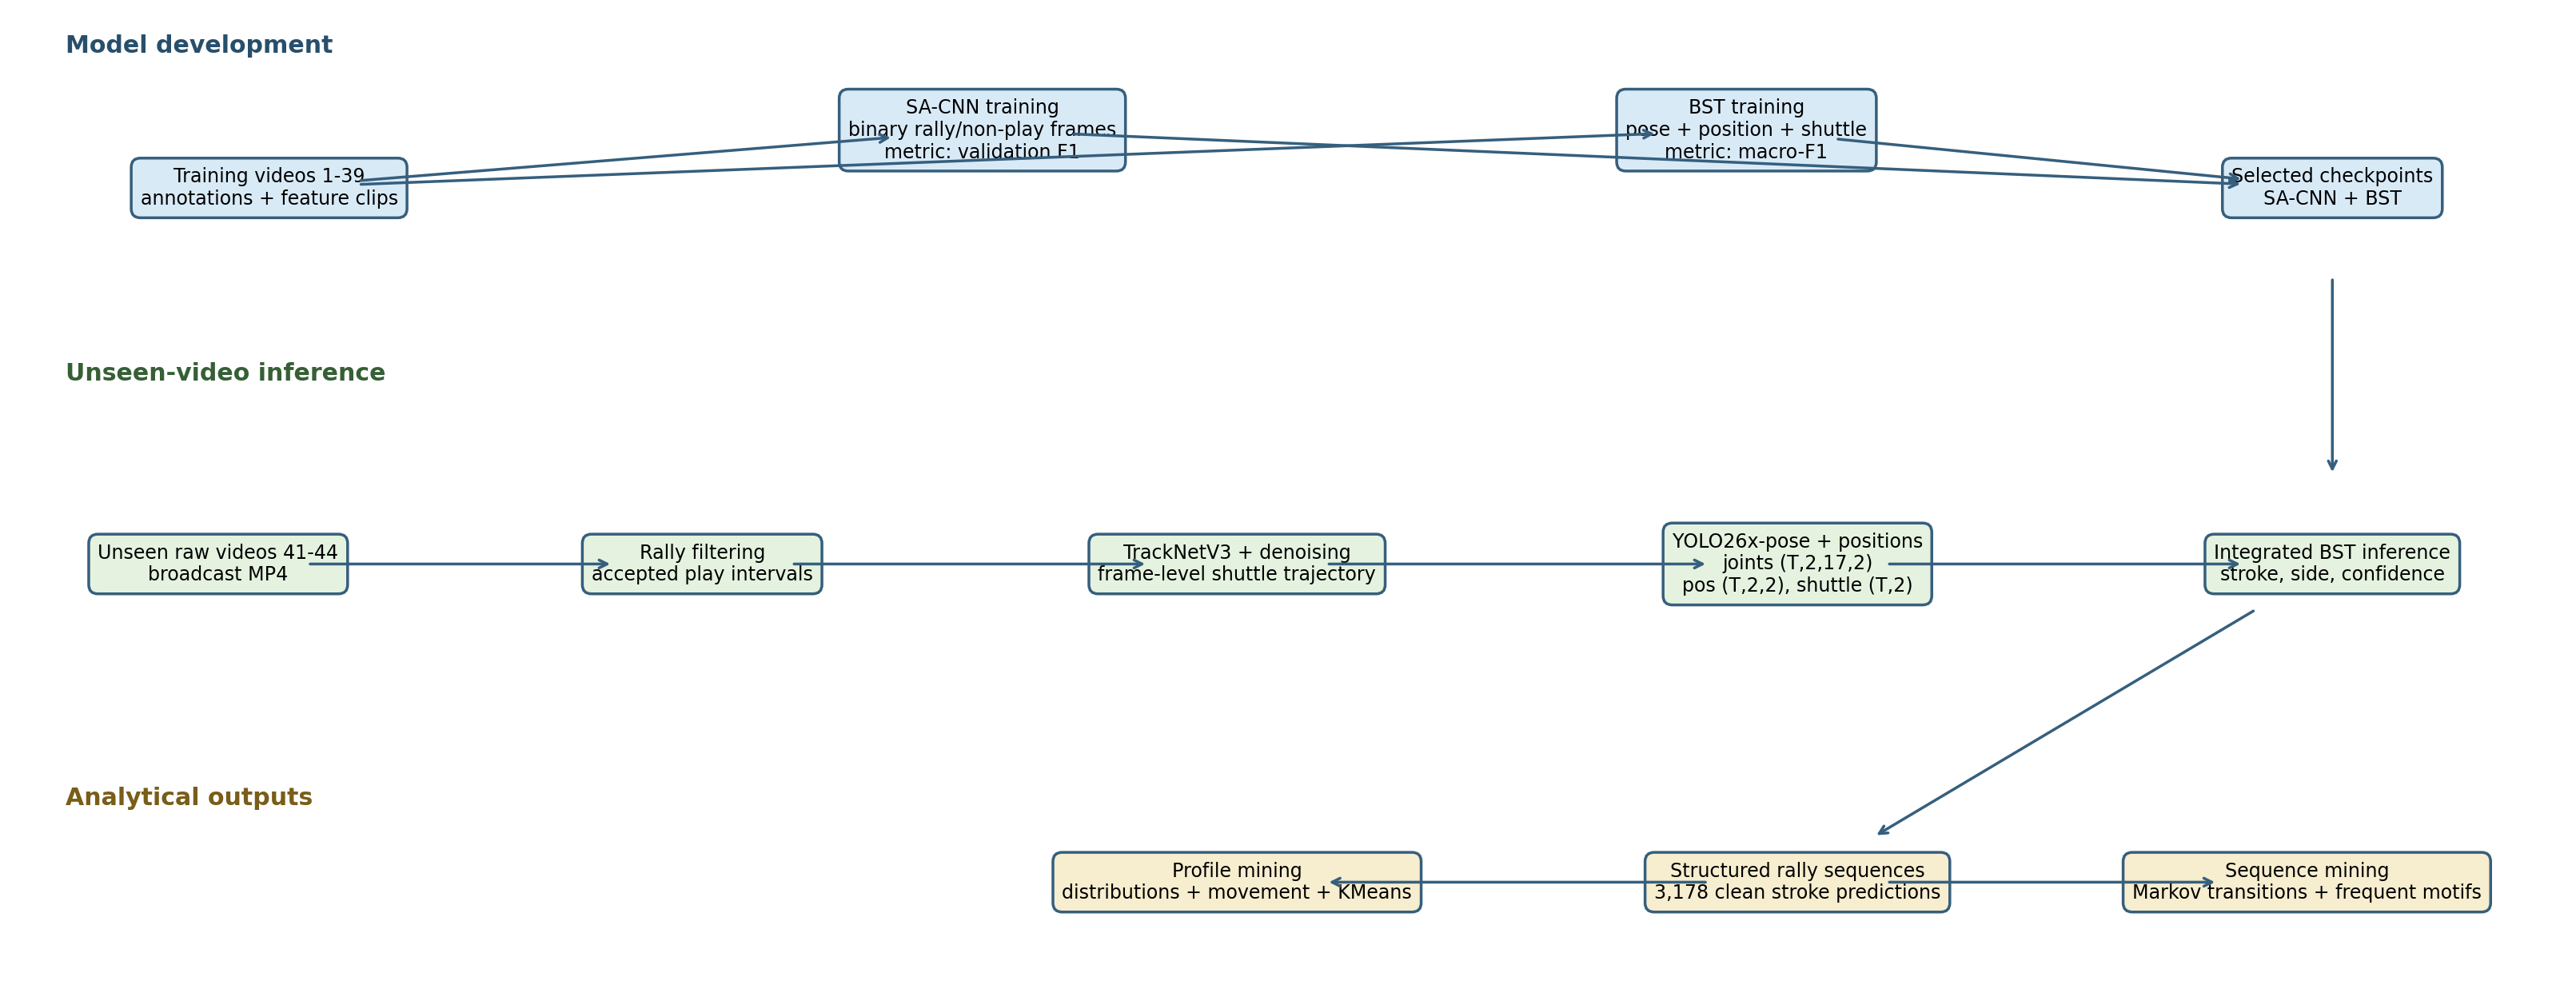
\includegraphics[width=0.98\textwidth]{raw_video_workflow.png}
  \caption{\textbf{System overview.} Models are developed from videos 1--39
  and applied to unseen broadcast videos 41--44. The predicted structured
  stroke sequence is the common input to tactical mining. Exact hit labels and
  supplied homographies are used to construct and score the current benchmark;
  fully label-free deployment requires automatic hit detection and new-video
  court calibration.}
  \label{fig:workflow}
\end{figure*}

\section{Related Work}

\paragraph{Badminton datasets and structured analysis.}
ShuttleSet provides match metadata, per-stroke annotations, court
homographies, and pre-extracted pose, position, and shuttle features
\cite{shuttleset}. Its annotations make it possible to evaluate both
stroke-level prediction and tactical patterns. BadmintonDB instead emphasizes
player-specific analysis and prediction \cite{badmintondb}. Our work uses
ShuttleSet because it contains both full broadcast video and the structured
labels needed to measure end-to-end error propagation.

\paragraph{Shuttle and hitting-event detection.}
TrackNetV2 formulates shuttle tracking as heatmap prediction over consecutive
frames \cite{tracknetv2}; the local TrackNetV3 implementation adds attention
and is used here as the frame-level shuttle estimator. Chen~\cite{chen2023hitting}
studies hitting-event detection from video clips. Our active benchmark uses
exact annotated hit frames to isolate the quality of feature extraction and
stroke classification, while retaining a trajectory-based detector for
fully unlabeled deployment.

\paragraph{Pose and stroke recognition.}
MMPose provides a modular pose-estimation toolbox \cite{mmpose}. For the active
run, we use a YOLO26x-pose checkpoint for efficient player pose extraction and
temporal tracking. BST models racket-sport strokes from skeleton, player
position, and shuttle sequences \cite{chang2025bst}. We fine-tune its
\texttt{BST\_CG\_AP} variant and reproduce its sequence-100 joint-plus-bone
input contract.

\paragraph{Data mining from predicted event streams.}
Distribution analysis summarizes tactical composition; Markov transition
models capture local sequential dependence; and frequent contiguous patterns
reveal longer tactical motifs. Movement profiles connect normalized positions
and displacement with stroke choices. KMeans clustering \cite{kmeans} and
silhouette analysis \cite{silhouette} provide exploratory grouping of those
profiles. Our distinguishing focus is to run this five-stage mining analysis
on a predicted event stream, compare it with annotation-derived references,
and quantify which tactical structures survive upstream perception noise.

\section{Problem Formulation}

Let a broadcast video be a frame sequence
$V=(I_1,\ldots,I_F)$. The system must produce an ordered set of stroke events
\[
\hat{\mathcal{E}} =
\{(v,r,k,f_k,\hat{s}_k,\hat{c}_k,q_k)\}_{k=1}^{N},
\]
where $v$ is video identity, $r$ is rally identity, $k$ is event rank,
$f_k$ is the event frame, $\hat{s}_k$ is one of 25 side-aware stroke classes,
$\hat{c}_k$ is confidence, and $q_k$ contains feature-quality measurements.
Each class encodes both camera-relative hitter side and merged stroke type.

Given the ordered event stream, tactical mining estimates:
\begin{enumerate}[leftmargin=*,nosep]
  \item stroke-type distributions by video and hitter side;
  \item a transition matrix
  $P_{ij}=P(\hat{s}_{t+1}=j\mid\hat{s}_t=i)$;
  \item frequent contiguous motifs and their rally support;
  \item player-set movement-strategy profiles; and
  \item exploratory KMeans groups of player or video-side profiles.
\end{enumerate}

The benchmark uses raw frames from videos 41--44 for shuttle, pose, feature,
and class prediction. Exact ShuttleSet hit frames and supplied homographies
construct reference windows and court normalization. Consequently, this is an
unseen-video raw-feature benchmark, but not yet fully label-free arbitrary
video inference.

\section{Method}

\subsection{From Video to a Mineable Event Table}

The perception stack is an enabling stage rather than the analytical endpoint.
Its purpose is to convert video into a relational event table with one ordered
row per stroke. Table~\ref{tab:pipeline-contracts} summarizes the contracts
that connect the stages. Rally filtering removes non-play footage; TrackNetV3
estimates and denoises shuttle trajectories; YOLO26x-pose extracts and
temporally associates the two players; and a fine-tuned BST classifier maps
the resulting sequence representation to a 25-class side-aware stroke
distribution. For a clip of length $T$, the representation contains joints
$J\in\mathbb{R}^{T\times2\times17\times2}$, player positions
$X\in\mathbb{R}^{T\times2\times2}$, and shuttle coordinates
$B\in\mathbb{R}^{T\times2}$. Nineteen bone vectors are appended to the 17
joints and the sequence is padded or sampled to length 100.

\begin{table*}[t]
  \caption{Perception stages and their role in tactical mining. The benchmark
  uses supplied exact hit frames and homographies; these two inputs are not
  predicted by the current unseen-video experiment.}
  \label{tab:pipeline-contracts}
  \centering
  \small
  \begin{tabular}{p{0.16\textwidth}p{0.22\textwidth}p{0.25\textwidth}p{0.27\textwidth}}
    \toprule
    Stage & Input & Output used by mining & Principal quality risk \\
    \midrule
    Rally filtering & Broadcast frames & Accepted play intervals & Close-ups
    and replays can contaminate interval boundaries. \\
    Shuttle tracking & Three-frame windows & Denoised frame-aligned shuttle
    coordinates & A visible prediction is not necessarily the true shuttle. \\
    Stroke windows & Exact hit frames in the current benchmark & Ordered,
    rally-aligned event windows & Deployment requires automatic hit detection. \\
    Court normalization & Supplied homography & Normalized player and shuttle
    coordinates & Deployment requires calibration for each new camera view. \\
    Pose and tracking & Event-window frames & Two ordered pose streams,
    positions, and validity masks & The far-side player is small and frequently
    missing. \\
    Stroke recognition & Length-100 multimodal sequence & Class probabilities,
    top-1 label, and confidence & Similar fine-grained strokes remain confusable. \\
    \bottomrule
  \end{tabular}
\end{table*}

The resulting event table is
$\hat{\mathcal{E}}=\{(v,r,k,f_k,\hat{s}_k,\mathbf{p}_k,\hat{c}_k,
\mathbf{x}_k,\mathbf{q}_k)\}$, where $\mathbf{p}_k$ is the full class
probability vector, $\mathbf{x}_k$ contains normalized spatial measurements,
and $\mathbf{q}_k$ records feature validity. This table is the common input to
all mining methods below. Keeping probabilities and quality metadata alongside
the top-1 prediction is essential: it allows us to determine whether a pattern
is robust, merely frequent, or concentrated in low-quality observations.

\subsection{Stroke Distribution Profiling}

\paragraph{Input and computation.}
The simplest tactical view aggregates top-1 stroke labels by camera-relative
hitter side. For side $a$ and stroke type $j$, we compute count
$n_{a,j}$ and within-side frequency
$d_{a,j}=n_{a,j}/\sum_\ell n_{a,\ell}$. We also compute the global
\emph{none} rate to diagnose whether the event stream is sufficiently complete
for sequence mining.

\paragraph{Output, utility, and limitation.}
The distribution reveals which actions dominate the recovered matches and
provides an immediate class-imbalance and integration diagnostic. It is useful
for deciding which tactical relations have enough support for further study.
However, Top and Bottom identify camera sides, not persistent athletes. Their
frequencies mix tactics, player identity, opponent response, and perception
quality; therefore, raw side differences are not interpreted as intrinsic
player styles.

\paragraph{Observed insight.}
The predicted stream is dominated by returns, drops, clears, lobs, pushes, and
smashes, but the large Top/Bottom pose-quality gap prevents interpreting the
side-level differences as a player taxonomy.

\subsection{Markov Transition Mining}

\paragraph{Input and computation.}
Within each rally, ordered adjacent strokes form directed transitions. Hard
counts are
\[
C_{ij}=\sum_r\sum_{t=1}^{|r|-1}
\mathbb{1}[\hat{s}_{r,t}=i,\hat{s}_{r,t+1}=j],
\qquad
P_{ij}=\frac{C_{ij}}{\sum_j C_{ij}}.
\]
The row-normalized matrix $P$ estimates the next-stroke distribution
conditioned on the current stroke. We compare hard top-1 transitions with two
alternatives. The soft estimator accumulates outer products
$\sum_{r,t}\mathbf{p}_{r,t}\mathbf{p}_{r,t+1}^{\top}$, retaining classifier
uncertainty. The high-confidence estimator keeps only contiguous transitions
whose two events satisfy $\hat{c}\geq0.8$. Each predicted matrix is compared
with the exact-label matrix using Frobenius distance and mean row-wise KL
divergence.

\paragraph{Output and tactical use.}
Transition heatmaps expose local attack--response structure, such as whether a
lift is followed by a smash or a smash by a defensive return. They can support
coaching questions about expected replies and expose where a player or system
deviates from common response patterns. Comparing estimators also answers a
data-mining question: whether uncertainty weighting improves aggregate
structure when individual labels are noisy.

\paragraph{Limitation.}
A first-order Markov model deliberately ignores rally history and score
context. Rare rows yield unstable estimates, while confidence filtering can
break valid rallies into short fragments. Soft probabilities help only when
they are calibrated; diffuse or systematically biased probability mass can
blur rather than recover strong transitions.

\paragraph{Observed insight.}
Hard predictions recover the strongest lift--attack and smash--defense
relations and substantially outperform the earlier integrated baseline. Soft
aggregation blurs these relations, while confidence filtering sacrifices too
much sequence coverage.

\subsection{Frequent Contiguous Motif Mining}

\paragraph{Input and computation.}
To capture structures longer than one transition, each rally is represented as
a side-aware stroke string. For a contiguous motif $m$ of length $n$, we count
at most one occurrence per rally and define rally support
\[
\operatorname{support}(m)=
\frac{|\{r:m\text{ occurs contiguously in }r\}|}{|\mathcal{R}|}.
\]
We enumerate recurrent $n$-grams in both the exact-label and predicted streams.
The former supports tactical conclusions; agreement in the latter measures
whether those structures survive the integrated pipeline. A separate
ground-truth opening analysis conditions point outcome on the first three
strokes after service.

\paragraph{Output and tactical use.}
Motifs turn a large transition matrix into readable tactical phrases. Coaches
can retrieve rallies exhibiting a common construction, compare alternative
third shots after service, or identify frequently repeated attack--defense
sequences. Side-aware motifs additionally preserve the direction of exchange.

\paragraph{Limitation.}
Exact contiguous matching fragments semantically similar tactics when one
stroke is mislabeled or inserted. High-support motifs describe prevalence, not
causal effectiveness. Outcome claims are restricted to the exact-label opening
analysis because the current prediction stream does not infer point winner.

\paragraph{Observed insight.}
The exact-label stream exposes a recurring net-shot $\rightarrow$ lob
$\rightarrow$ smash $\rightarrow$ defensive-reply grammar. The predicted
stream recovers its shorter components, but errors increasingly fragment
longer motifs.

\subsection{Movement Strategy Profiles}

\paragraph{Input and computation.}
Supplied homographies first map valid player positions into a normalized
player-centric half-court, so movement direction has the same meaning across
camera sides. For each player-set profile with at least 30 valid events, we
aggregate 12
interpretable measurements: mean forward location; lateral and forward
location variability; mean inter-stroke displacement; rates of rightward,
netward, and right-baselineward displacement; smash/net-attack and lift/clear
rates; smash after large displacement; and rear-court smash rate. This produces
16 player-set profiles from 2,300 valid events and 1,710 displacement pairs;
four low-support profiles are excluded. ShuttleSet A/B identity and true side
are used to link events within a set.

\paragraph{Output and tactical use.}
Profiles combine where a player acts, how much the player moves between events,
and which strokes follow those movements. They support exploratory comparisons
such as whether forward movement is associated with attacking actions. We also
report feature correlations, treating them as descriptive associations rather
than causal relationships.

\paragraph{Limitation.}
Inter-stroke displacement is a coarse endpoint measurement, not footwork.
Profiles can mix opponent pressure, score state, and camera quality with player
preference. The identity link relies on ShuttleSet metadata; deployment on a
new broadcast requires persistent player re-identification.

\paragraph{Observed insight.}
Netward displacement is positively associated with smash rate, whereas
right-baselineward displacement is negatively associated. These moderate
correlations suggest testable movement--attack relationships, not causal rules.

\subsection{KMeans Clustering and Stability Analysis}

\paragraph{Input and computation.}
We standardize profile features and apply KMeans \cite{kmeans} to three
granularities: exact-label player-match profiles, predicted video-side
profiles, and extended movement profiles. Candidate values of $k$ are compared
using silhouette score \cite{silhouette}, minimum cluster size, and bootstrap
adjusted Rand index (ARI). The bootstrap procedure repeatedly resamples the
data and measures whether memberships remain consistent.

\paragraph{Output, utility, and limitation.}
Clustering is used as an exploratory summarizer, not as proof of universal
player archetypes. A useful partition must be separated, stable, and
non-degenerate. Low silhouette or ARI indicates that apparent groups are
sensitive to sampling or overlap strongly. Predicted video-side clusters can
also encode video quality or camera domain rather than tactics, so cluster
names are withheld unless supported by stronger evidence.

\paragraph{Observed insight.}
All selected clusterings have low silhouette and moderate-to-low bootstrap
stability. The current data supports exploratory profile comparison, but not a
stable vocabulary of universal player styles.

\section{Experimental Setup}

\subsection{Dataset and Protocol}

The local ShuttleSet snapshot contains 44 raw broadcast videos, 104 set-level
CSV files, 36,482 annotated strokes, and 3,683 rallies. Six pre-extracted
feature variants each contain 33,481 clips. We use the merged, 2D,
between-hit sequence-100 variant with 25 side-aware classes.

\begin{table}[t]
  \caption{Dataset and evaluation summary.}
  \label{tab:data}
  \centering
  \small
  \begin{tabular}{lr}
    \toprule
    Item & Count / split \\
    \midrule
    Raw broadcast videos & 44 \\
    Annotated strokes / rallies & 36,482 / 3,683 \\
    Prepared feature clips & 33,481 \\
    BST train / validation clips & 25,741 / 4,241 \\
    Development videos & 1--39 \\
    Unseen evaluation videos & 41--44 \\
    Clean unseen predictions & 3,178 \\
    \bottomrule
  \end{tabular}
\end{table}

Videos 1--39 support training, development, and parameter selection. Videos
41--44 are designated as the unseen-video evaluation set. Video 40 appears in
intermediate shuttle and window outputs but is not part of the final
integrated bundle. The inherited reference feature split historically places
video 41 in validation; we disclose this and retain videos 42--44 as a stricter
secondary subset.

\subsection{Baselines and Metrics}

\paragraph{Baselines.}
The principal systems baseline is the earlier integrated Phase 09 pipeline,
which produced 2,986 labeled predictions, 8.41\% accuracy, and a 56.43\%
\emph{none} prediction rate. For tactical mining, we compare hard, soft, and
high-confidence transition estimators against exact labels. Annotation-derived
patterns and profiles serve as references, not deployable predictions.

\paragraph{Metrics.}
Stroke classification uses side-aware top-1 accuracy, top-3 accuracy,
player-side accuracy, stroke-type accuracy ignoring side, and supported-class
macro-F1. Rally filtering reports validation F1, annotated-hit coverage, and
rally overlap. Shuttle tracking reports visible-frame coverage before and
after denoising. Distribution and motif mining report counts, proportions, and
rally support. Movement profiling reports valid-event coverage and feature
correlations. Clustering reports silhouette and bootstrap ARI. Tactical
sequence fidelity uses transition Frobenius error and mean row KL.

\subsection{Implementation Details}

All project-owned stages are implemented in Python and PyTorch. BST is
initialized from the ShuttleSet \texttt{BST\_CG\_AP} checkpoint and fine-tuned
with class-weighted cross entropy, label smoothing 0.05, AdamW, learning rate
$5\times10^{-5}$, cosine scheduling, gradient clipping, and early stopping on
validation macro-F1. Training uses sequence length 100 and batch size 128.
SA-CNN is trained for 20 epochs with batch size 64. The tracked pose run uses
YOLO26x-pose at image size 640, half precision, batch size 128, and two GPUs.
All phases emit CSV/JSON summaries and preserve source paths and runtime
configuration where available.

\section{Results}

\subsection{Component Performance}

\begin{table}[t]
  \caption{Component-level results. ``Coverage'' is the fraction of frames
  with a visible shuttle prediction.}
  \label{tab:components}
  \centering
  \small
  \begin{tabular}{llr}
    \toprule
    Component & Metric & Result \\
    \midrule
    BST & Best validation macro-F1 & 0.805 \\
    SA-CNN & Best validation F1 & 0.903 \\
    SA-CNN & Annotated-hit coverage & 97.32\% \\
    TrackNet & Raw coverage, videos 40--44 & 86.63\% \\
    TrackNet & Denoised coverage, videos 40--44 & 90.99\% \\
    Pose & Top / Bottom pose-valid rate & 54.29 / 98.96\% \\
    Pose & Both-player pose-missing rate & 0.85\% \\
    \bottomrule
  \end{tabular}
\end{table}

The models are individually operational, but Table~\ref{tab:components}
exposes a major asymmetry: the far-side Top player is missing in almost half
of frames, while the near-side Bottom player is nearly always visible.
TrackNet denoising improves visibility by 4.36 percentage points and produces
no visible out-of-range coordinates.

\begin{figure}[t]
  \centering
  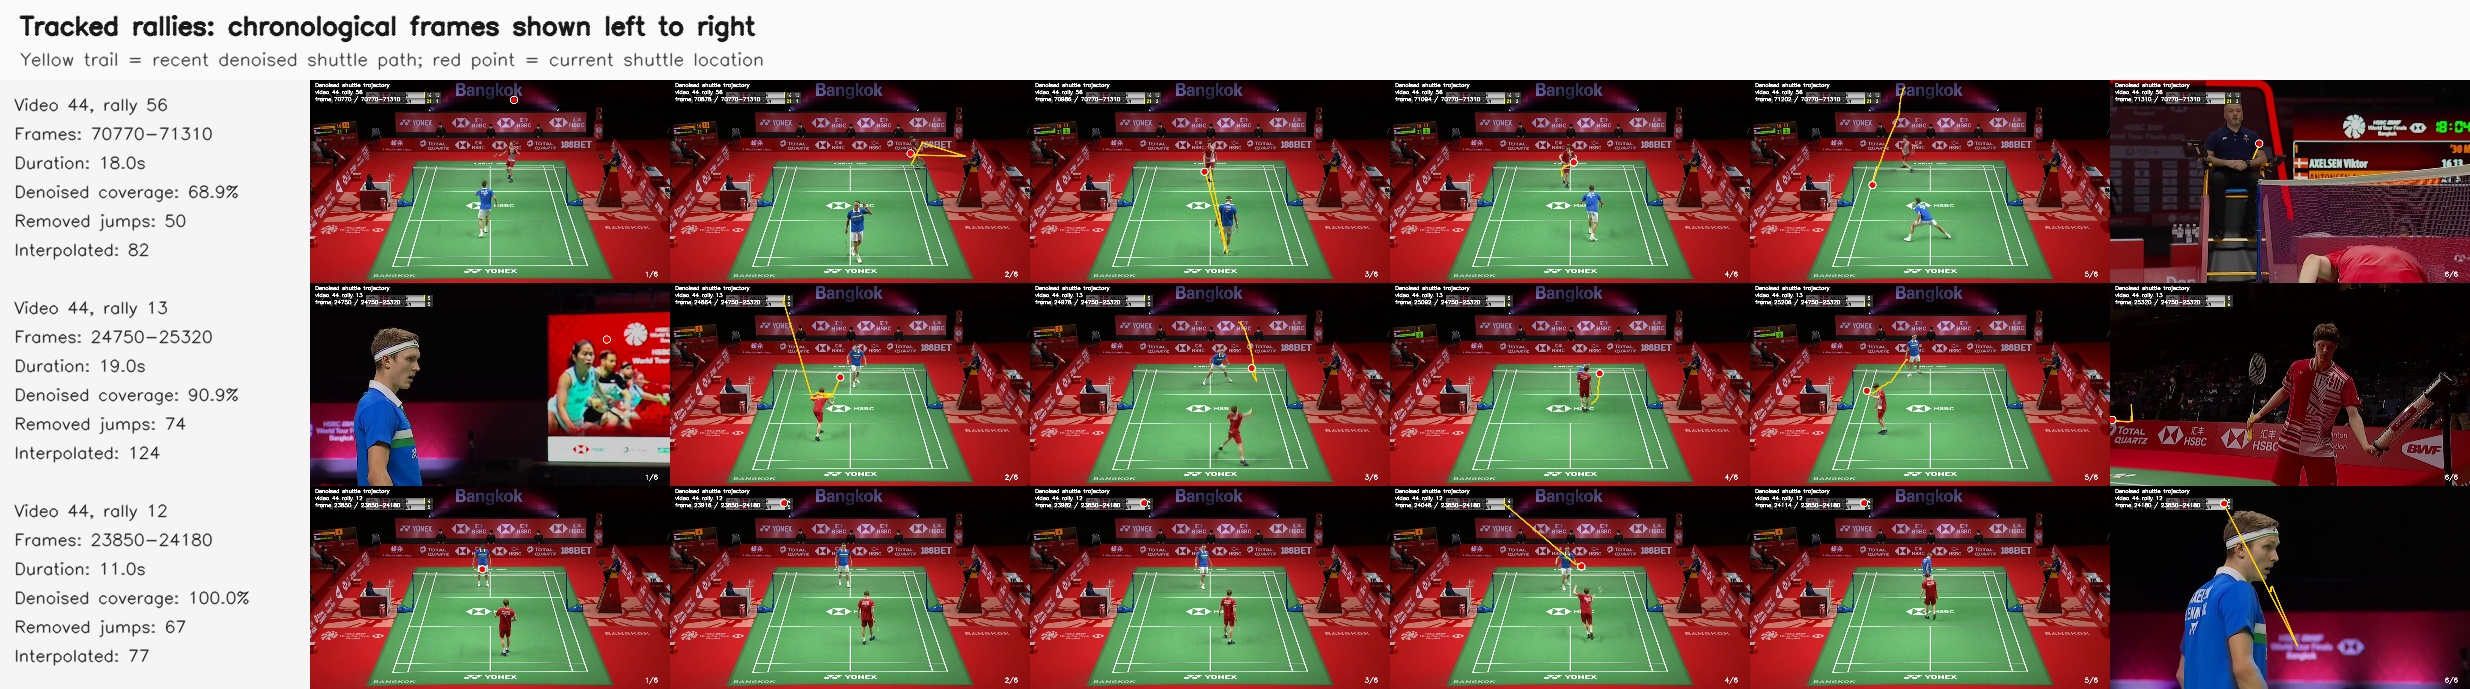
\includegraphics[width=\linewidth]{tracked_rally_examples.jpg}
  \caption{\textbf{Qualitative shuttle tracking.} Yellow trails are denoised
  trajectories and red points are current shuttle positions. Post-rally
  close-ups in final frames reveal that high coverage does not guarantee
  precise rally boundaries.}
  \label{fig:tracking}
\end{figure}

\subsection{Unseen-Video Stroke Classification}

\begin{table}[t]
  \caption{Integrated classification on clean unseen videos 41--44. The
  inherited 42--44 subset is included for reproducibility.}
  \label{tab:classification}
  \centering
  \small
  \begin{tabular}{lrr}
    \toprule
    Metric & Videos 41--44 & Videos 42--44 \\
    \midrule
    Rows & 3,178 & 2,027 \\
    Side-aware top-1 & \textbf{69.04\%} & 66.40\% \\
    Top-3 & \textbf{87.89\%} & 86.43\% \\
    Player-side accuracy & \textbf{93.05\%} & 92.06\% \\
    Stroke-type accuracy & \textbf{69.19\%} & 66.60\% \\
    Supported macro-F1 & \textbf{66.64\%} & 64.07\% \\
    \bottomrule
  \end{tabular}
\end{table}

The gap between player-side accuracy and full side-aware accuracy indicates
that the system usually identifies the hitter's court side, while fine stroke
distinctions remain difficult. Performance also varies substantially by
video: side-aware accuracy is 73.68\%, 63.97\%, 53.27\%, and 76.57\% for
videos 41--44, respectively.

\begin{figure}[t]
  \centering
  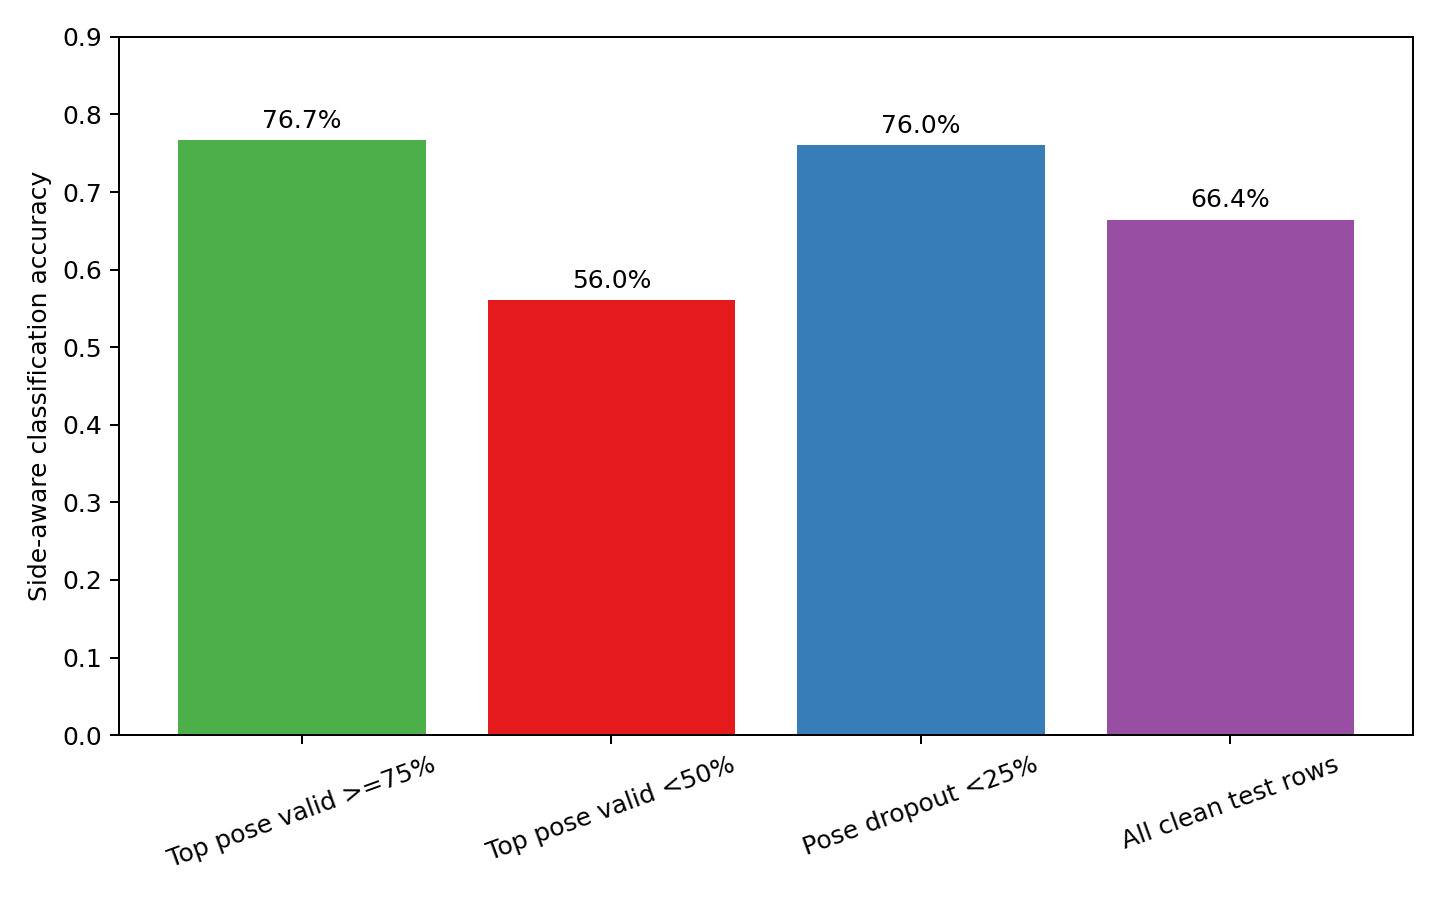
\includegraphics[width=\linewidth]{accuracy_by_feature_quality.png}
  \caption{\textbf{Accuracy by feature quality on the strict 42--44 subset.}
  Accuracy reaches 76.71\% when Top-player pose validity is at least 75\%, but
  falls to 56.05\% when it is below 50\%.}
  \label{fig:quality}
\end{figure}

Figure~\ref{fig:quality} gives the strongest system-level diagnosis. Better
far-side features correspond to a 20.66 percentage-point accuracy gain. This
effect is larger and more actionable than differences between downstream
mining algorithms.

\subsection{Stroke Distribution Analysis}

The clean predicted stream contains 3,178 strokes over 343 rallies, compared
with 36,482 strokes over 3,683 rallies in the complete annotation-derived
reference. Its mean rally length is 9.27 strokes, close to the reference mean
of 9.91. More importantly, the \emph{none} rate is 6.70\%, down from 56.43\%
in the earlier integrated baseline. This reduction restores the continuity
required by transition and motif mining.

The most frequent predicted Bottom-side strokes are return net (210), drop
(199), clear (166), lob (161), and push (160). For Top, smash (232), lob
(207), clear (182), net shot (173), and drop (136) dominate. The contrast is
descriptively useful, but it cannot be interpreted as a stable player-style
difference: Top/Bottom are camera-relative roles, and the Top stream has much
lower pose validity. The counts therefore expose both tactical composition and
the risk of perception-induced distribution shift.

\begin{figure}[t]
  \centering
  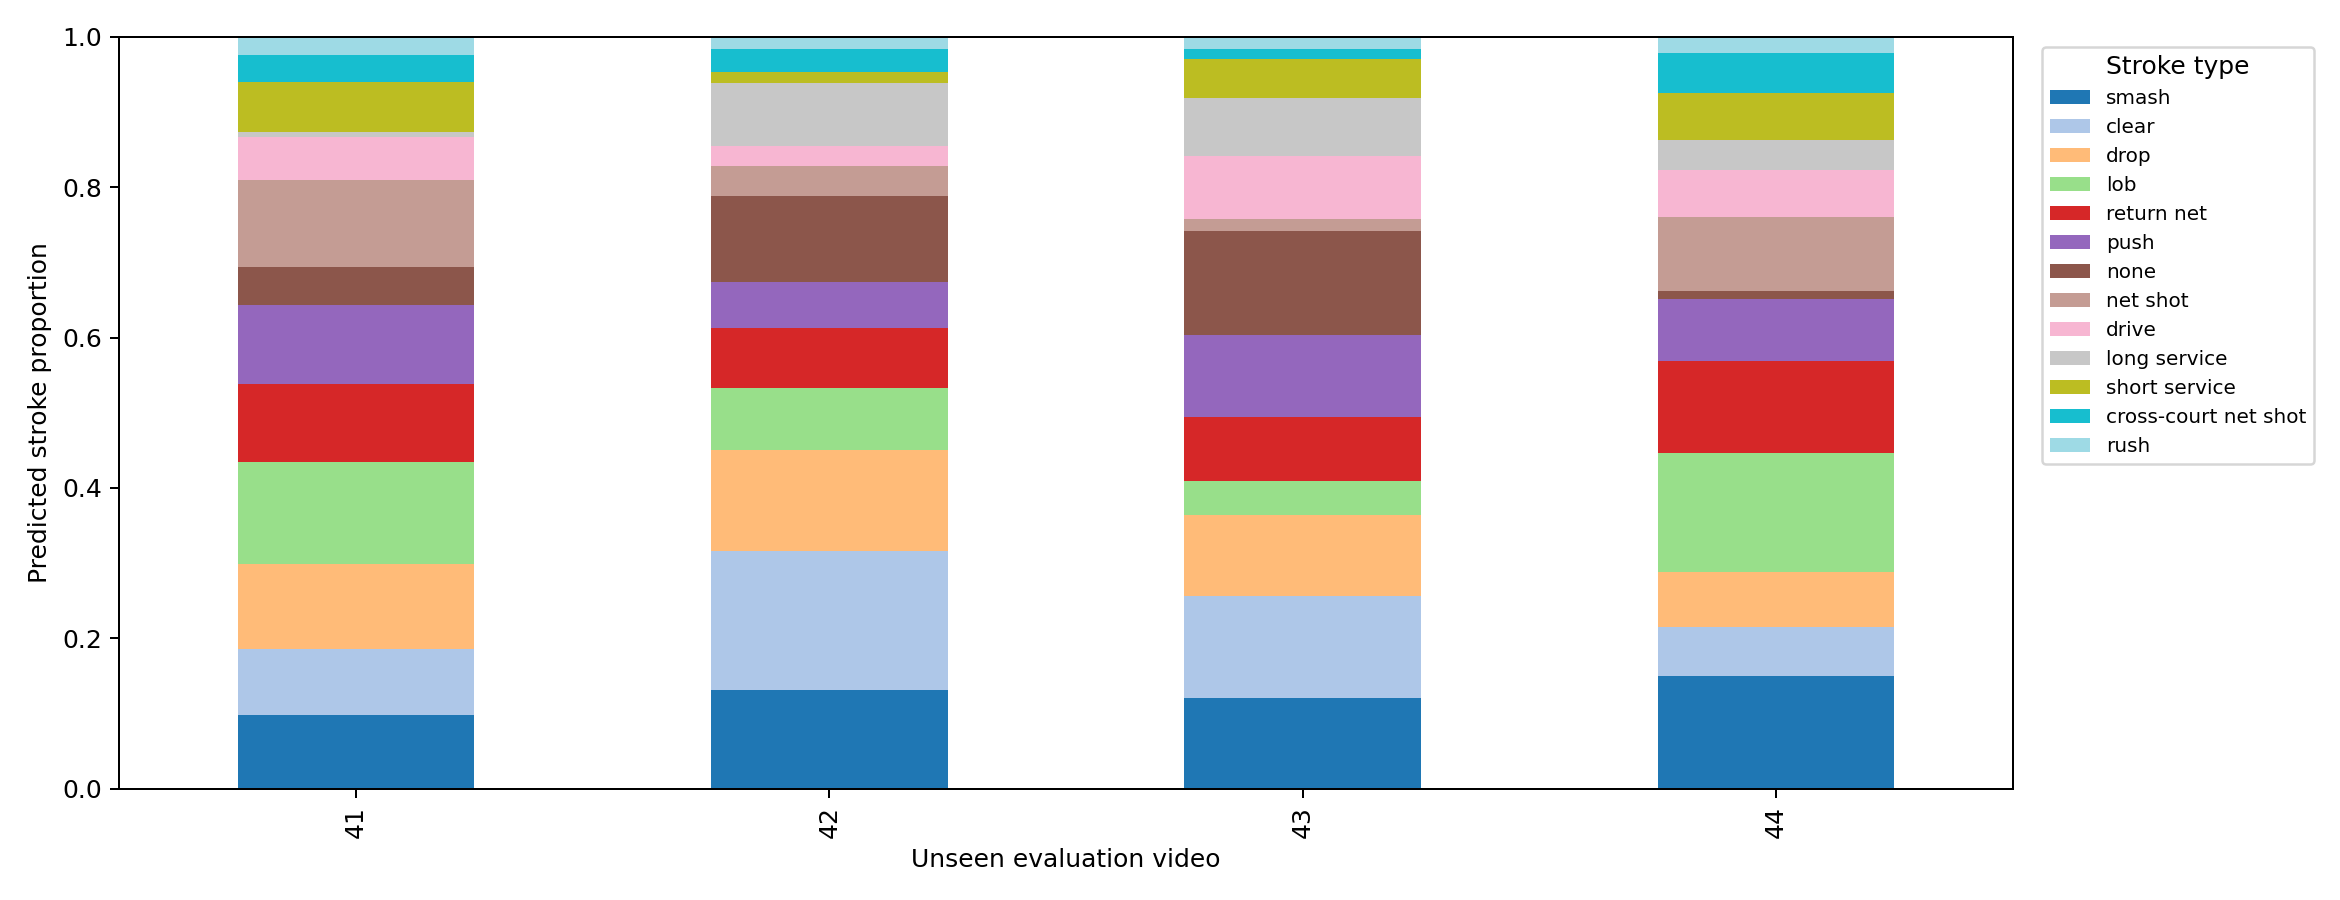
\includegraphics[width=\linewidth]{predicted_stroke_distributions.png}
  \caption{\textbf{Predicted stroke distributions by unseen video.} Stroke
  composition varies across matches, but these differences can reflect both
  tactics and perception quality.}
  \label{fig:distributions}
\end{figure}

\subsection{Markov Transition Analysis}

\begin{table}[t]
  \caption{Transition-matrix error against exact unseen-video labels. Lower is
  better.}
  \label{tab:transition}
  \centering
  \small
  \begin{tabular}{lrr}
    \toprule
    Estimator & Frobenius & Mean row KL \\
    \midrule
    Earlier integrated baseline & 3.652 & 11.723 \\
    Current hard predictions & \textbf{1.232} & \textbf{0.511} \\
    Current soft probabilities & 1.617 & 0.623 \\
    High-confidence segments & 1.211 & 1.372 \\
    \bottomrule
  \end{tabular}
\end{table}

The current hard transition matrix reduces Frobenius error by 66.3\% and mean
row KL by 95.6\% relative to the earlier pipeline. This is the clearest
evidence that the recovered event stream is useful for mining even though its
individual labels are imperfect. Strong lift--attack and smash--defense
relations remain visible. Soft transitions perform worse because residual
probability mass blurs these concentrated relations. High-confidence segments
have slightly lower Frobenius error, but their row KL is substantially worse:
low coverage removes entire response categories and makes rare rows unstable.
Confidence is therefore used as a Markov-analysis ablation rather than a
separate mining algorithm.

\begin{figure*}[t]
  \centering
  \begin{minipage}[t]{0.49\textwidth}
    \centering
    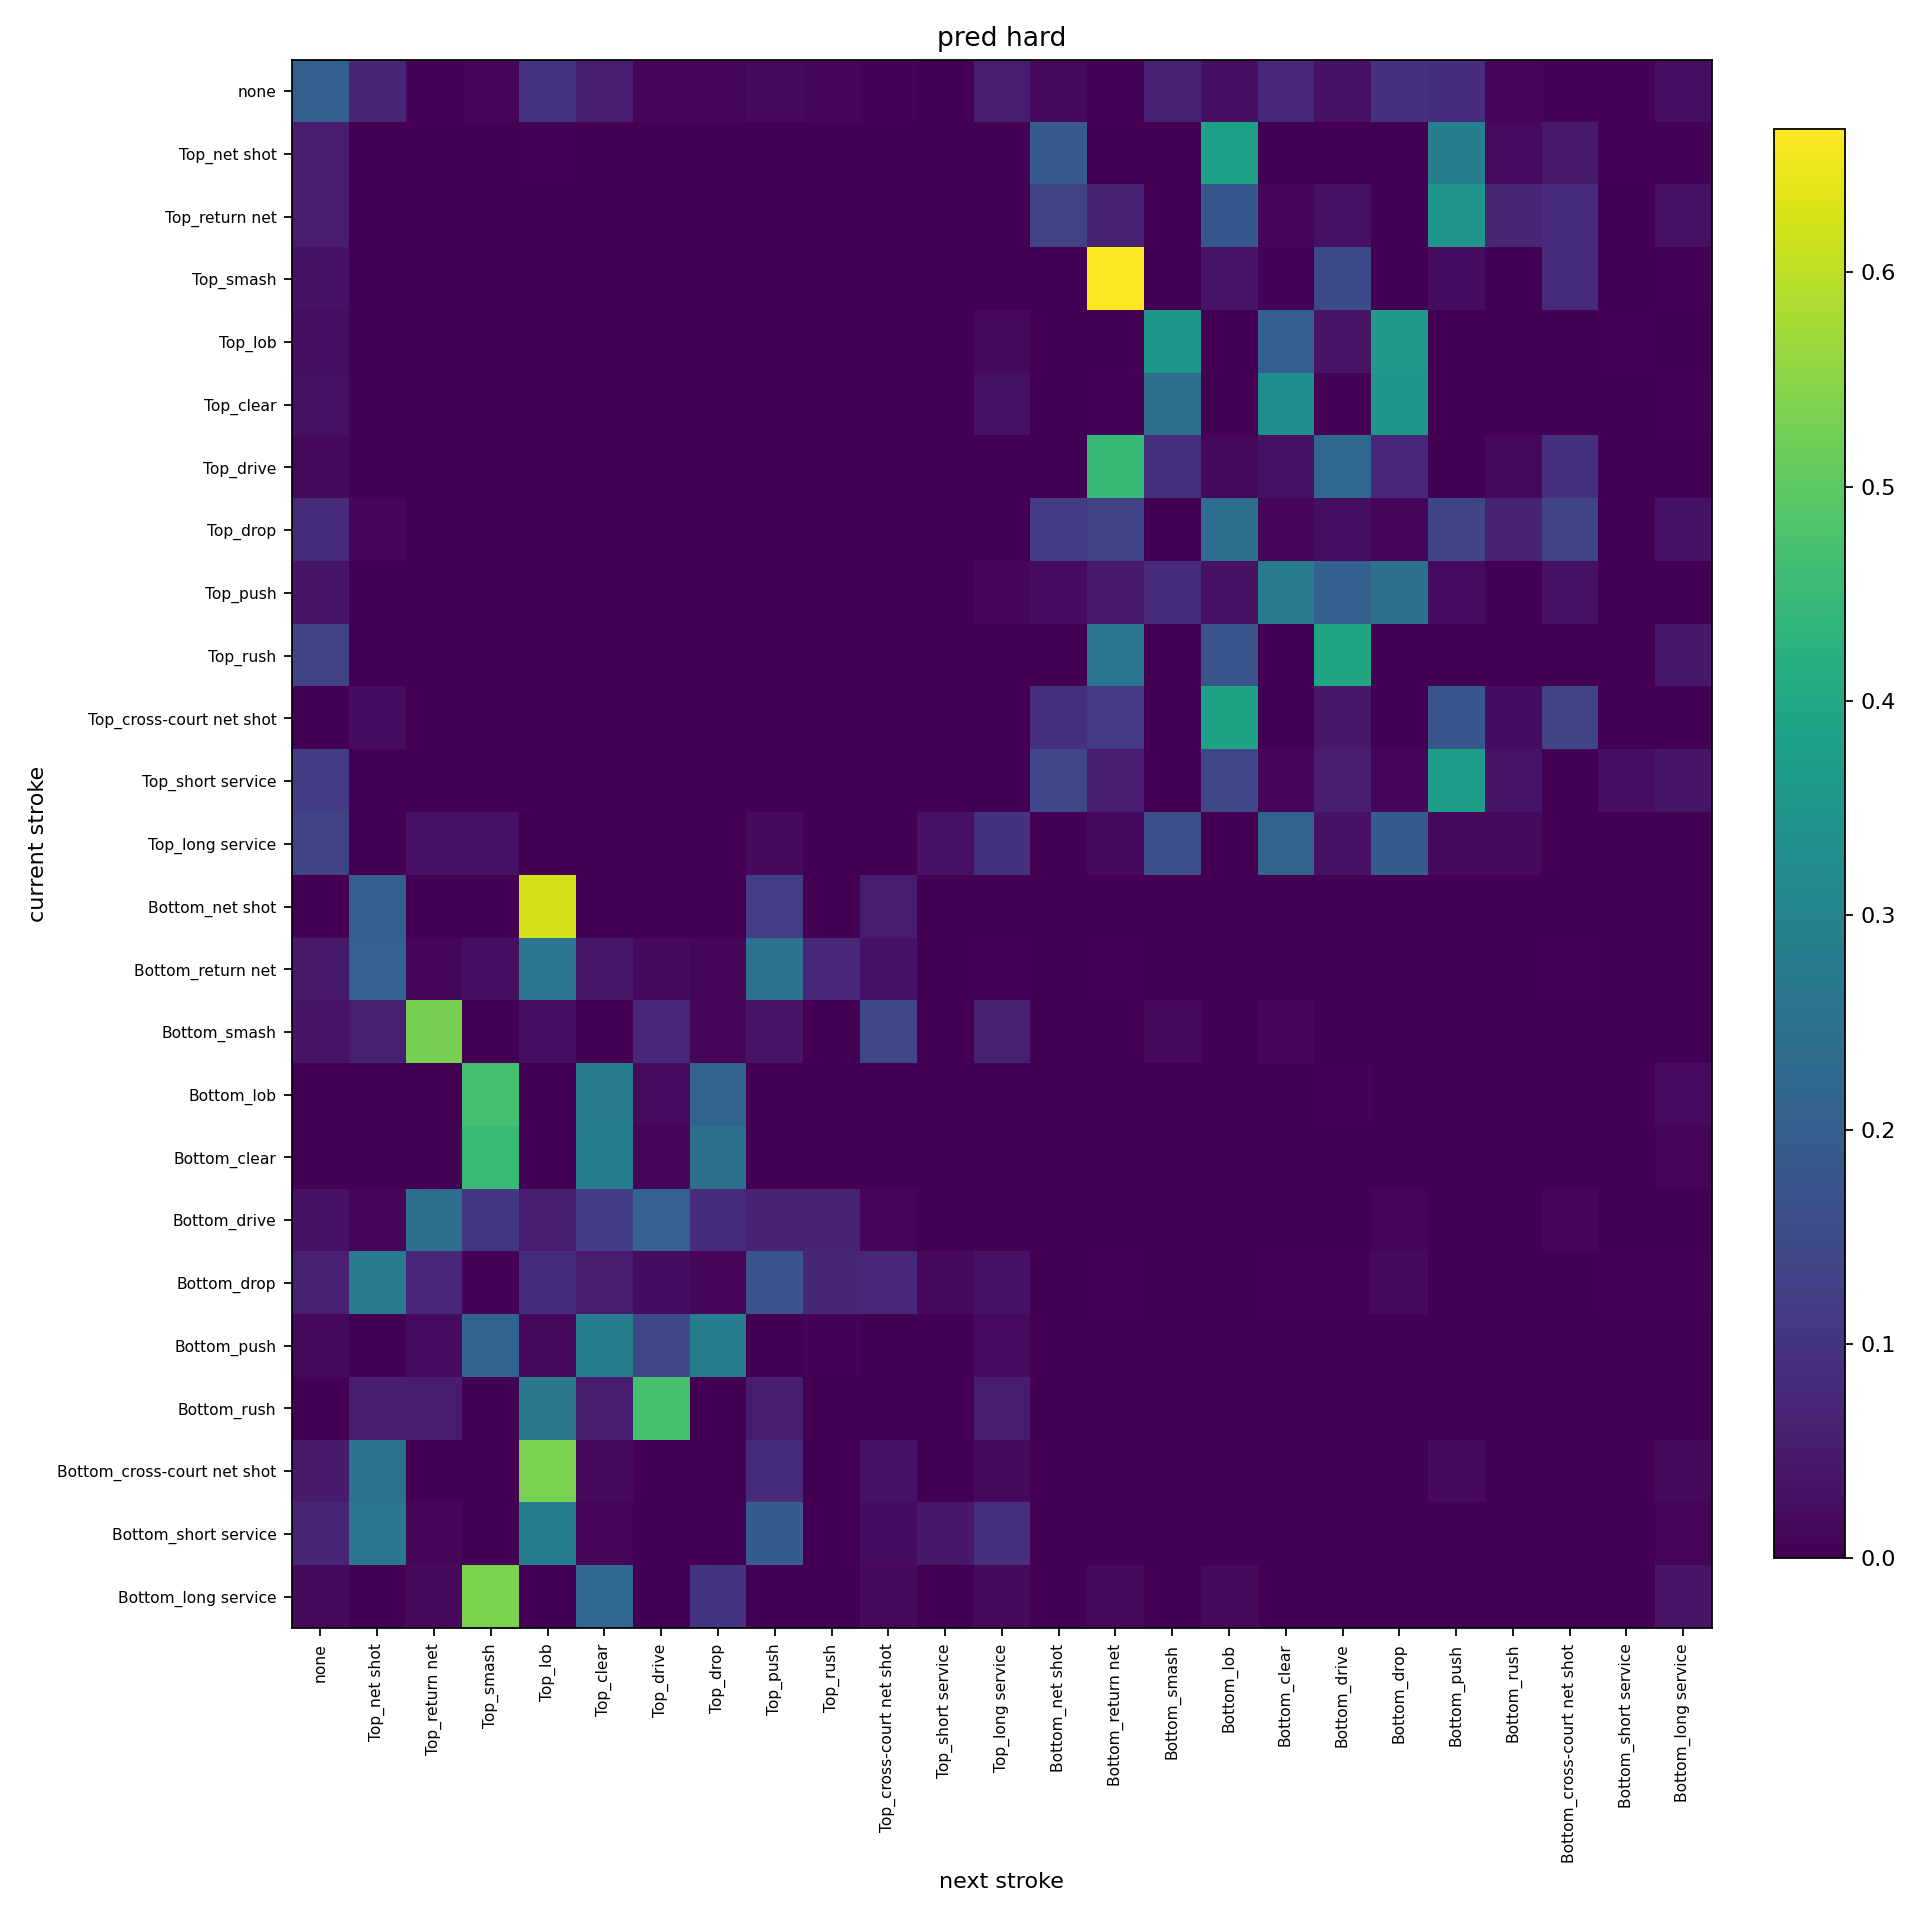
\includegraphics[width=\linewidth]{predicted_transition_heatmap.png}
    \small (a) Predicted hard-transition matrix.
  \end{minipage}
  \hfill
  \begin{minipage}[t]{0.49\textwidth}
    \centering
    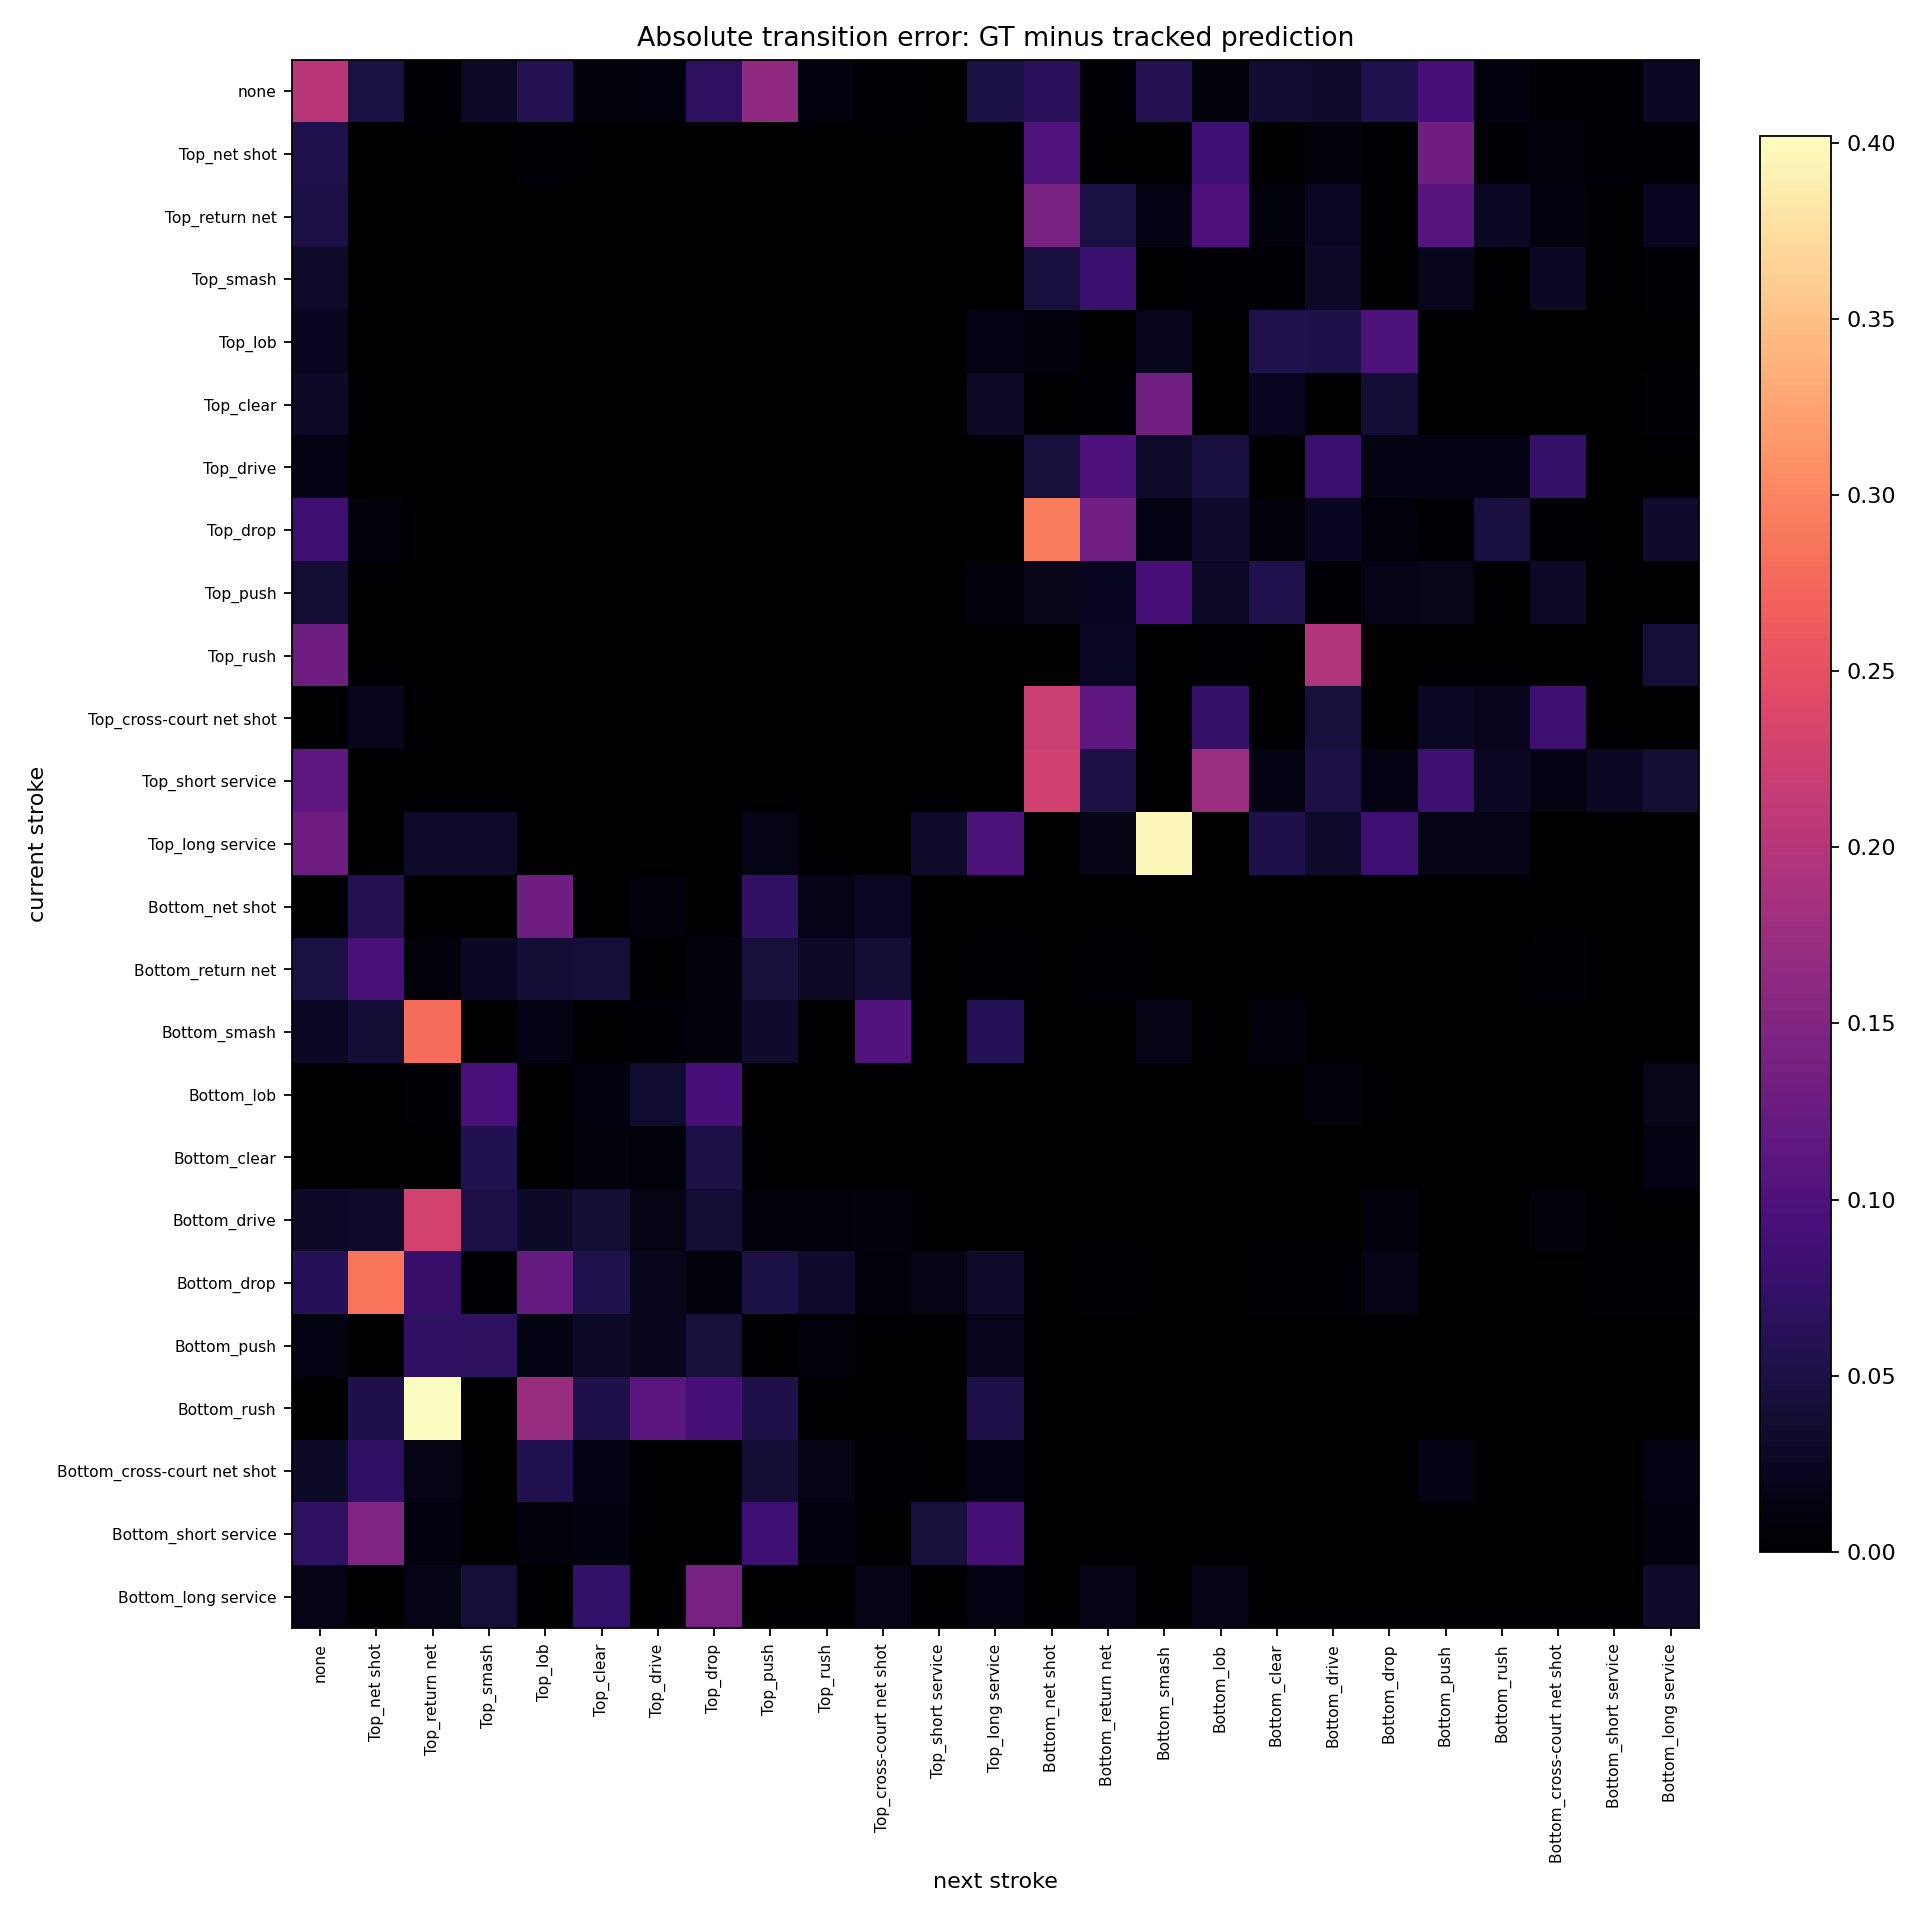
\includegraphics[width=\linewidth]{transition_error_heatmap.png}
    \small (b) Absolute error relative to exact labels.
  \end{minipage}
  \caption{\textbf{Tactical transition recovery.} The predicted stream
  preserves strong smash--defense and lift--attack relations. Remaining error
  concentrates around finer net, push, drop, rush, and service distinctions.}
  \label{fig:transitions}
\end{figure*}

\subsection{Frequent Motif Mining}

The annotation-derived stream reveals a recurring attack--defense grammar:
\[
\text{net shot}\rightarrow\text{lob}\rightarrow
\text{smash}\rightarrow\text{defensive net}.
\]
The complete four-stroke motif appears in 11.16\% of rallies; its
\emph{net shot $\rightarrow$ lob} and \emph{smash $\rightarrow$ defensive
net} sub-patterns appear in 48.76\% and 30.30\%, respectively. The predicted
stream recovers the side-aware four-stroke counterpart
\emph{Top net shot $\rightarrow$ Bottom lob $\rightarrow$ Top smash
$\rightarrow$ Bottom return net} in 4.66\% of unseen-video rallies.

Ground-truth opening patterns further show that the third shot matters:
\emph{short service $\rightarrow$ push $\rightarrow$ clear} has a 37.50\%
server win rate, compared with 53.52\% for
\emph{short service $\rightarrow$ lob $\rightarrow$ smash} and 60.00\% for
\emph{short service $\rightarrow$ lob $\rightarrow$ tap smash}. These
outcome-based conclusions are ground-truth-only because the prediction path
does not infer point winners.

The shorter predicted motifs show which parts of this grammar survive
perception noise. \emph{Top smash $\rightarrow$ Bottom return net} appears in
28.86\% of predicted rallies; \emph{Bottom lob $\rightarrow$ Top smash} in
18.08\%; \emph{Bottom clear $\rightarrow$ Top smash} in 17.49\%; and
\emph{Bottom smash $\rightarrow$ Top return net} in 15.45\%. The predicted
three-stroke sequence \emph{Top net shot $\rightarrow$ Bottom lob
$\rightarrow$ Top smash} retains 7.58\% support. Together, these motifs show
that the event stream preserves a readable attack--defense exchange, while the
drop from 11.16\% exact-label support to 4.66\% predicted support for the full
four-stroke motif quantifies how quickly classification errors fragment longer
patterns.

\subsection{Movement Strategy Profiling}

The profiling stage produces 16 player-set profiles from 2,300 valid events
and 1,710 inter-stroke displacement pairs; four sparse profiles are excluded.
The mean lateral coordinate
is 0.496 and the mean forward coordinate is 0.450. Furthermore, 58.43\% lie
in the central lateral corridor, 71.22\% lie in the middle-depth band, and
46.65\% lie in their intersection. These position summaries form part of the
movement profiles and are consistent with central-base positioning at stroke
time, but they do not measure continuous recovery movement.

Movement profiles provide cautious evidence that displacement direction and
attack choice are related. Netward displacement has a positive correlation
with smash rate ($r=0.304$), whereas right-baselineward displacement has a
negative correlation ($r=-0.335$). These associations are consistent with
forward pressure preceding attack and retreat reducing immediate smash
opportunity, but they are not causal and can reflect opponent behavior.

\subsection{KMeans Clustering}

\begin{figure}[t]
  \centering
  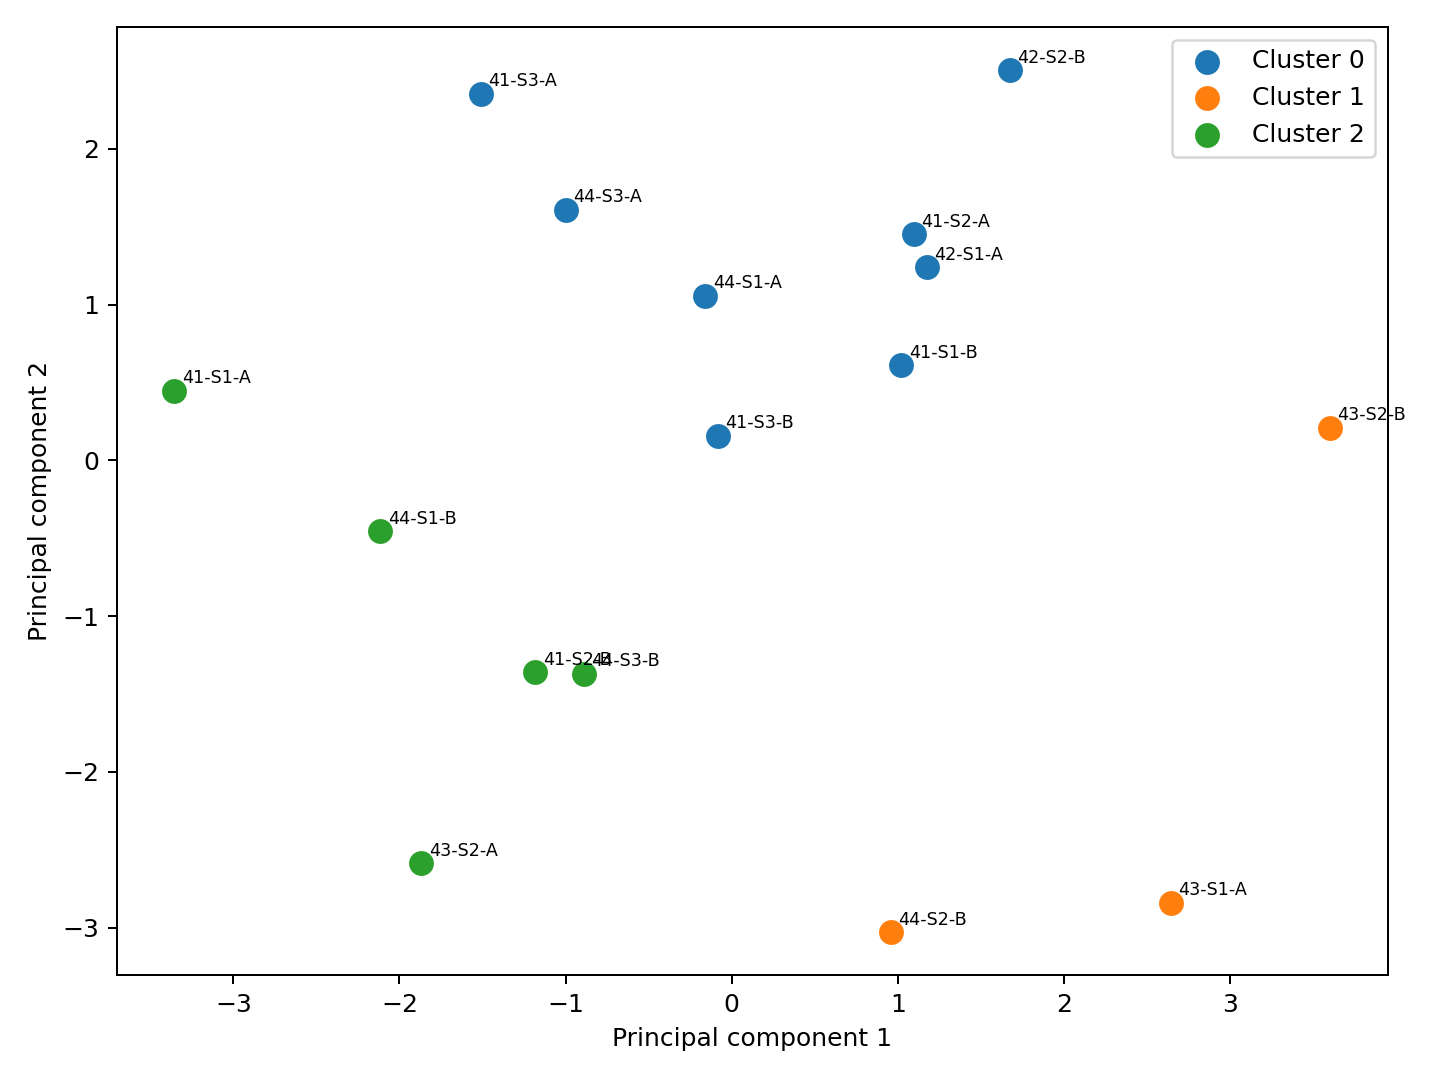
\includegraphics[width=\linewidth]{movement_strategy_clusters.png}
  \caption{\textbf{KMeans movement-profile clustering.} Substantial overlap
  and isolated points explain the weak silhouette and stability results;
  clusters are exploratory rather than stable player archetypes.}
  \label{fig:clustering}
\end{figure}

KMeans clustering is less conclusive. The selected exact-label player-match solution
uses $k=2$ over 88 profiles and obtains
silhouette 0.152 and bootstrap ARI 0.440. Predicted video-side profiles obtain
silhouette 0.200 and ARI 0.505 for $k=2$ over only eight units, but primarily
separate video domains rather than player styles; a $k=3$ solution is rejected
because it contains a singleton. Extended movement profiles select $k=3$ and
obtain silhouette 0.151 and ARI 0.365, with a minimum cluster size of three.
These values do not justify naming universal player archetypes. The negative
finding is itself useful: the available sample supports descriptive profiling,
but not strong claims about discrete strategy types.

\section{Discussion and Originality}

The project's originality lies in converting separate research assets into a
reproducible data mining system and evaluating the \emph{quality of the mined
structure}, not only component accuracy. Project-owned scripts build normalized
ground-truth tables, collate 33,481 feature triples, fine-tune BST and SA-CNN,
wrap TrackNet inference and denoising, generate validity-aware tracked pose
features, repair simultaneous-event aliases, and produce structured tactical
outputs. This integration creates a new evaluation setting for the local
ShuttleSet snapshot.

Five findings summarize the selected algorithms. First, stroke distributions
provide a compact match-level tactical summary but remain sensitive to
camera-side quality. Second, sequence-level improvement is larger than top-1
accuracy alone suggests: the \emph{none} rate falls from 56.43\% to 6.70\%,
allowing Markov transitions and recognizable motifs to reappear. Third, hard
predictions preserve transitions better than soft probability accumulation.
Fourth, movement profiles reveal moderate, non-causal movement--attack
associations. Fifth, KMeans groups overlap too strongly to justify a universal
player-style taxonomy. Reliable far-side features still raise accuracy by over
20 percentage points, so perception quality must qualify conclusions from all
five algorithms.

\section{Limitations}

The unseen-video benchmark uses supplied ShuttleSet hit frames and
homographies; it is not fully label-free arbitrary-video inference. Video 41
historically belongs to the inherited reference-validation split, although
this project designates videos 41--44 as its unseen evaluation bundle and
reports the inherited 42--44 subset separately. Only four unseen videos
contribute to predicted tactical mining. Fourteen simultaneous-event aliases
are excluded from clean evaluation.

The pipeline does not predict point winner, win/loss reason, exact shuttle
landing, or persistent player identity. Inter-stroke displacement is not
continuous footwork. Approximate shuttle endpoints are not physical landing
positions. Finally, high shuttle and rally coverage do not guarantee precise
rally boundaries; qualitative review still reveals post-rally close-ups.

\section{Conclusion}

We presented \method, an integrated badminton video analytics and data mining
system. On unseen ShuttleSet videos 41--44, the system achieves 69.04\%
side-aware top-1 accuracy and recovers transition and motif structure that was
destroyed by the earlier baseline. The analysis demonstrates that predicted
event streams can support stroke-distribution analysis, Markov transitions,
frequent motif mining, movement-strategy profiling, and exploratory KMeans
clustering when temporal alignment, player ordering, and feature quality are
explicitly controlled. The strongest
next steps are better far-side player extraction, tighter rally boundaries,
trajectory-based hit detection, new-video court calibration, and evaluation
beyond the supplied ShuttleSet metadata bundle.

\section*{Code Availability}

The final COMP4040 submission must include a repository or code archive link:
\codeurl. The repository contains project-owned phase scripts, configuration
and validation outputs; datasets and third-party model weights are excluded
from the submitted code package.

\section*{Team Contributions}

\textbf{Important before submission:} the rubric requires a verified
individual contribution statement. The repository does not contain enough
evidence to assign work fairly, so the team must replace the placeholders
below with the agreed contribution allocation.

\begin{itemize}[leftmargin=*]
  \item \textbf{Cao Pham Minh Dang:} \todo{describe verified individual
  contributions.}
  \item \textbf{Pham Dinh Hieu:} \todo{describe verified individual
  contributions.}
  \item \textbf{Pham Minh Hieu:} \todo{describe verified individual
  contributions.}
\end{itemize}

\section*{Acknowledgements}

No external collaboration or advisory contribution is documented in the
current project materials. The project builds on the open-source systems and
datasets cited below.

\bibliographystyle{plain}
\bibliography{reference}

\end{document}
